\pdfminorversion=4
\documentclass[aspectratio=169]{beamer}

\mode<presentation>
{
  \usetheme{default}
  \usecolortheme{default}
  \usefonttheme{default}
  \setbeamertemplate{navigation symbols}{}
  \setbeamertemplate{caption}[numbered]
  \setbeamertemplate{footline}[frame number]  % or "page number"
  \setbeamercolor{frametitle}{fg=white}
  \setbeamercolor{footline}{fg=black}
} 

\usepackage[english]{babel}
\usepackage[utf8x]{inputenc}
\usepackage{tikz}
\usepackage{courier}
\usepackage{array}
\usepackage{bold-extra}
\usepackage{minted}
\usepackage[thicklines]{cancel}
\usepackage{fancyvrb}

\xdefinecolor{dianablue}{rgb}{0.18,0.24,0.31}
\xdefinecolor{darkblue}{rgb}{0.1,0.1,0.7}
\xdefinecolor{darkgreen}{rgb}{0,0.5,0}
\xdefinecolor{darkgrey}{rgb}{0.35,0.35,0.35}
\xdefinecolor{darkorange}{rgb}{0.8,0.5,0}
\xdefinecolor{darkred}{rgb}{0.7,0,0}
\definecolor{darkgreen}{rgb}{0,0.6,0}
\definecolor{mauve}{rgb}{0.58,0,0.82}

\title[2022-03-18-awkward-cpp-for-atlas]{Integrating Awkward Array with C++ (potentially for Athena)}
\author{Jim Pivarski}
\institute{Princeton University -- IRIS-HEP}
\date{March 18, 2022}

\usetikzlibrary{shapes.callouts}

\begin{document}

\logo{\pgfputat{\pgfxy(0.11, 7.4)}{\pgfbox[right,base]{\tikz{\filldraw[fill=dianablue, draw=none] (0 cm, 0 cm) rectangle (50 cm, 1 cm);}\mbox{\hspace{-8 cm}\includegraphics[height=1 cm]{princeton-logo-long.png}\hspace{0.1 cm}\raisebox{0.1 cm}{\includegraphics[height=0.8 cm]{iris-hep-logo-long.png}}\hspace{0.1 cm}}}}}

\begin{frame}
  \titlepage
\end{frame}

\logo{\pgfputat{\pgfxy(0.11, 7.4)}{\pgfbox[right,base]{\tikz{\filldraw[fill=dianablue, draw=none] (0 cm, 0 cm) rectangle (50 cm, 1 cm);}\mbox{\hspace{-8 cm}\includegraphics[height=1 cm]{princeton-logo.png}\hspace{0.1 cm}\raisebox{0.1 cm}{\includegraphics[height=0.8 cm]{iris-hep-logo.png}}\hspace{0.1 cm}}}}}

% Uncomment these lines for an automatically generated outline.
%\begin{frame}{Outline}
%  \tableofcontents
%\end{frame}

% START START START START START START START START START START START START START

\begin{frame}{High-level overview}
\vspace{0.4 cm}
\begin{itemize}\setlength{\itemsep}{0.25 cm}
\item \textcolor{blue}{\href{https://inspirehep.net/literature/1806222}{Awkward Array}} is a library for end-user data analysts to interact with large datasets in Python.
\begin{itemize}
\item It's like NumPy, in that it's a collection of routines for {\it manipulating} arrays.
\item It's like Arrow, in that it represents arbitrary data types using a \textcolor{blue}{\href{https://arrow.apache.org/docs/format/Columnar.html}{columnar format}}.
\item \textcolor{blue}{\href{https://awkward-array.readthedocs.io/en/latest/ak.layout.Content.html}{Awkward Array's format}} is very similar to Arrow's; conversions are usually zero-copy.
\end{itemize}

\item<2-> Sits in the middle of an ecosystem of Pythonic tools:
\begin{itemize}
\item \textcolor{blue}{\href{https://pypi.org/project/uproot/}{Uproot}} reads ROOT data into Awkward Arrays.
\item \textcolor{blue}{\href{https://pypi.org/project/coffea/}{Coffea}} builds ROOT schema-specific extensions on top.
\item \textcolor{blue}{\href{https://pypi.org/project/vector/}{Vector}} implements array-oriented Lorentz vector operations.
\item \textcolor{blue}{\href{https://pypi.org/project/fastjet/}{fastjet}} (lowercase) runs FastJet (uppercase) on batches of events in Awkward Arrays.
\item \ldots
\end{itemize}

\item<3-> Interoperability with C++ is a priority, but ideas on how we'll do that \mbox{are evolving.\hspace{-1 cm}}
\begin{itemize}
\item Awkward 1.0 (late 2019) was implemented in C++ with the idea that downstream libraries would link to it. See \textcolor{blue}{\href{https://indico.cern.ch/event/855454/contributions/4605044/}{this talk}} for why that was a bad idea.
\item Awkward 2.0 (in \mintinline{python}{_v2} submodule) is implemented in Python without sacrificing speed (see page 7 in the above talk) or accessibility in C++ (this talk).
\end{itemize}

\end{itemize}
\end{frame}

\begin{frame}{Why the columnar format matters}
\large
\vspace{0.5 cm}
The large ``buffers'' of contiguous data are accessible in both C++ and Python.

\vspace{0.25 cm}
Only the small tree (number of nodes $\sim$ {\it data type}) combining them into a structure must be managed separately in C++ and Python.

\vspace{-0.25 cm}
\begin{columns}
\column{1.15\linewidth}
\only<1>{\includegraphics[width=\linewidth]{composable-1.pdf}}\only<2>{\includegraphics[width=\linewidth]{composable-2.pdf}}\only<3>{\includegraphics[width=\linewidth]{composable-3.pdf}}
\end{columns}
\end{frame}

\begin{frame}{Why the columnar format matters}
\vspace{0.35 cm}
\large

Record-oriented data can only be iterated over by procedures that are specialized to the data schema. For large-scale data, they must be compiled/JIT-compiled.

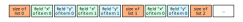
\includegraphics[width=\linewidth]{record-oriented.pdf}

\vspace{0.15 cm}
\begin{uncoverenv}<2->
Column-oriented data can be iterated over in two ways: (1)~precompiled routines that only operate on one column, or (2)~a JIT-compiled routine on whole records.

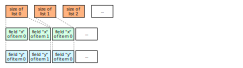
\includegraphics[width=\linewidth]{column-oriented.pdf}
\end{uncoverenv}

\vspace{-4 cm}
\hfill \begin{minipage}{0.45\linewidth}
\uncover<3->{In Awkward Array, the primary interface is a suite of array-at-a-time operations, precompiled and applied to a dynamically typed schema.}

\vspace{0.25 cm}
\uncover<4->{But we can also do record-at-a-time iteration if we have a JIT-compiler.}
\end{minipage}
\vspace{4 cm}
\end{frame}

\begin{frame}[fragile]{Record-at-a-time iteration without a JIT-compiler}
\vspace{0.1 cm}
\small
\begin{minted}{python}
array = ak._v2.from_parquet("zlib9-jagged3.parquet").tolist()
builder = ak._v2.ArrayBuilder()


def f_python(array, builder):
    out = 0.0
    for inner1 in array:
        for inner2 in inner1:
            for inner3 in inner2:
                for inner4 in inner3:
                    out += inner4
    builder.real(out)

starttime = time.time()
f_numba(array, builder)
print("Numba time", time.time() - starttime)   #  <--- 29.3 seconds

print("result", builder.snapshot()[0])
\end{minted}
\end{frame}

\begin{frame}[fragile]{Record-at-a-time iteration with a JIT-compiler: Numba}
\vspace{0.1 cm}
\small
\begin{minted}{python}
array = ak._v2.from_parquet("zlib9-jagged3.parquet")
builder = ak._v2.ArrayBuilder()

@nb.njit
def f_numba(array, builder):
    out = 0.0
    for inner1 in array:
        for inner2 in inner1:
            for inner3 in inner2:
                for inner4 in inner3:
                    out += inner4
    builder.real(out)

starttime = time.time()
f_numba(array, builder)
print("Numba time", time.time() - starttime)   #  <--- 1.72 seconds

print("result", builder.snapshot()[0])
\end{minted}
\end{frame}

\begin{frame}[fragile]{Record-at-a-time iteration with a JIT-compiler: Clang incremental}
\vspace{0.1 cm}
\small
\begin{minted}{python}
array = ak._v2.from_parquet("zlib9-jagged3.parquet")
builder = ak._v2.ArrayBuilder()

f_cpp = CppStatements("""
double out = 0.0;
for (auto inner1 : array) {
  for (auto inner2 : inner1) {
    for (auto inner3 : inner2) {
      for (auto inner4 : inner3) {
        out += inner4;
}}}} builder.real(out);
""", array=array, builder=builder)

starttime = time.time()
f_cpp(array=array, builder=builder)
print("C++   time", time.time() - starttime)   #  <--- 1.78 seconds

print("result", builder.snapshot()[0])
\end{minted}
\end{frame}

\end{document}
